\subsection{Moon gravity perturbation}
In this section, we investigate the effect of the moon's third body on satellite orbital elements. In this problem we calcualte forces of moon and earth, then, integrate from differential equation for several time to see effects in short, long period and secular.

$$
\sum F_{satellite} = \dfrac{-Gm_{earth}}{r_{e2s}^3} \boldsymbol{\mathrm{r_{e2s}}} + \dfrac{-Gm_{moon}}{r_{m2s}^3} \boldsymbol{\mathrm{r_{m2s}}}
$$
Here is the result of perturbation forces on
orbital elements. The simulation has been in the Jupyter notebook. the results are presented here.

\begin{figure}[H]
    \centering
    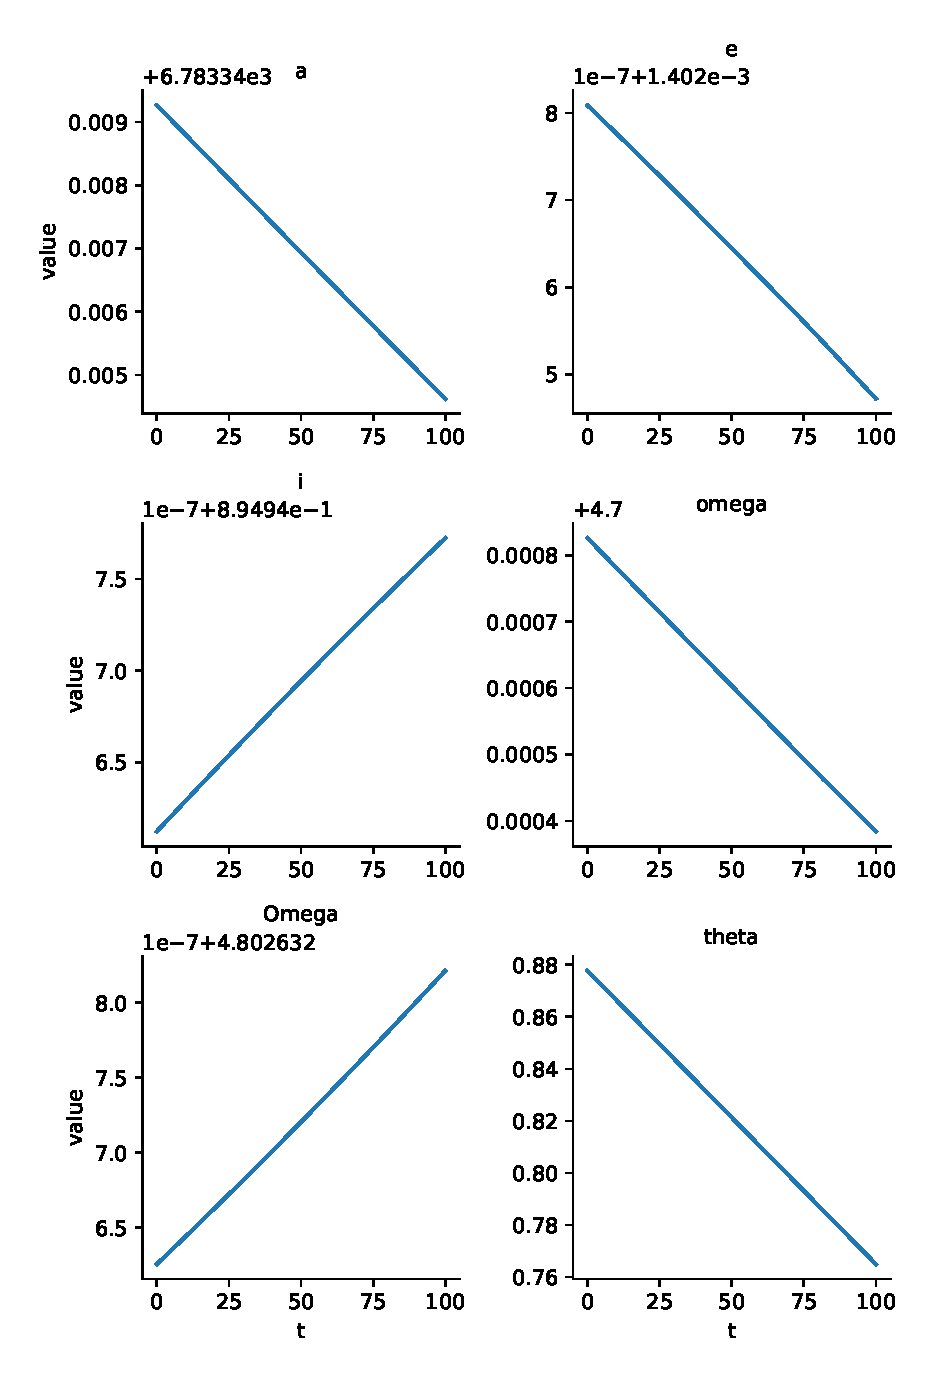
\includegraphics[width=0.85\textwidth]{../Figure/Q2/orbital_elements_variation_moon_100}
    \caption{Variation of Parameter due to moon gravity perturbation for 100 seconds}
\end{figure}


\begin{figure}[H]
    \centering
    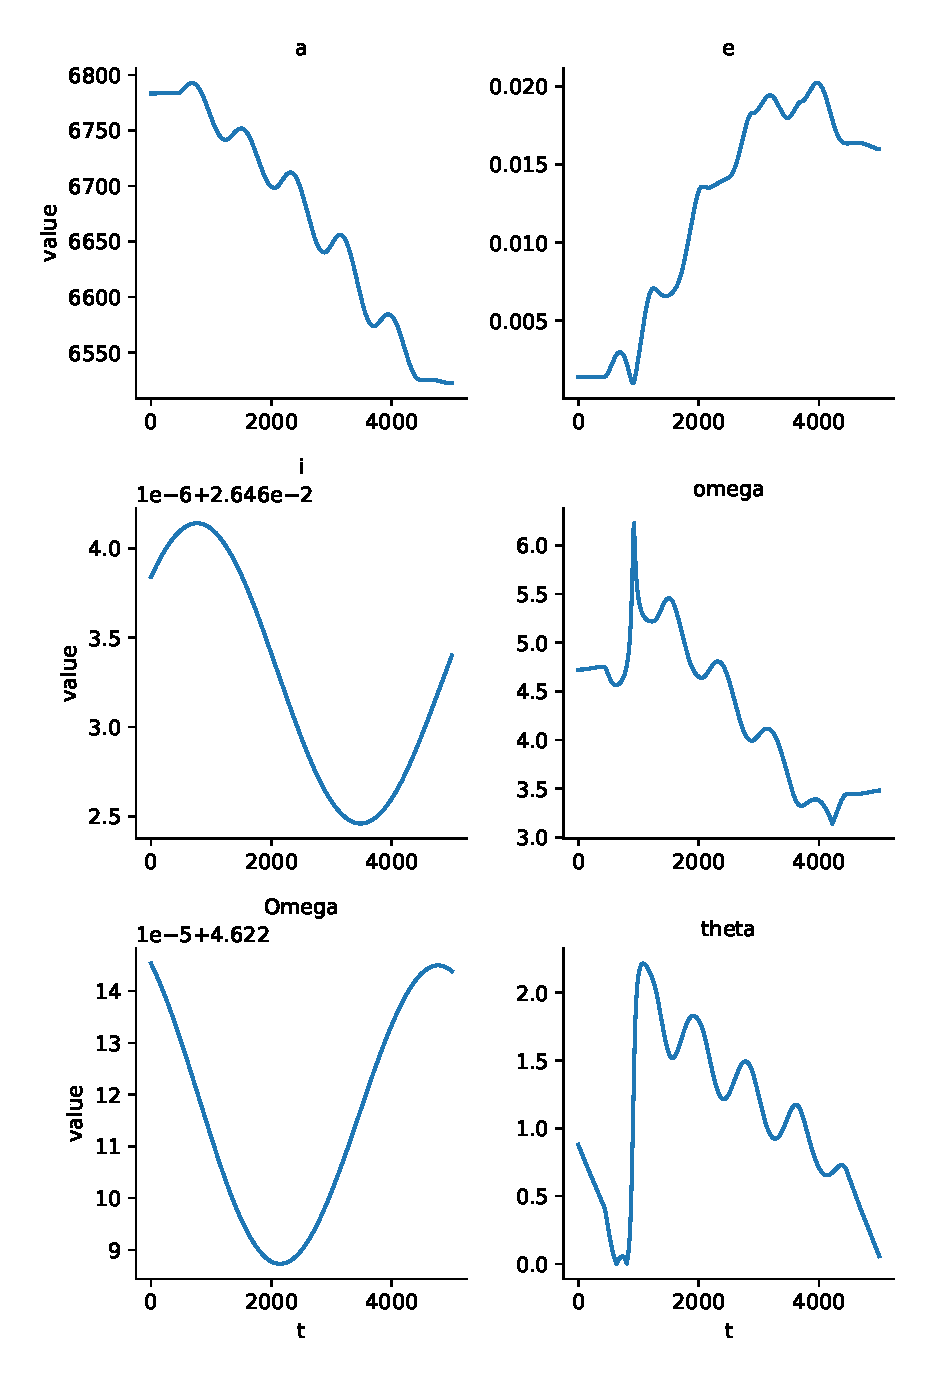
\includegraphics[width=0.85\textwidth]{../Figure/Q2/orbital_elements_variation_moon_5000}
    \caption{Variation of Parameter due to moon gravity perturbation for 5000 seconds}
\end{figure}

\begin{figure}[H]
    \centering
    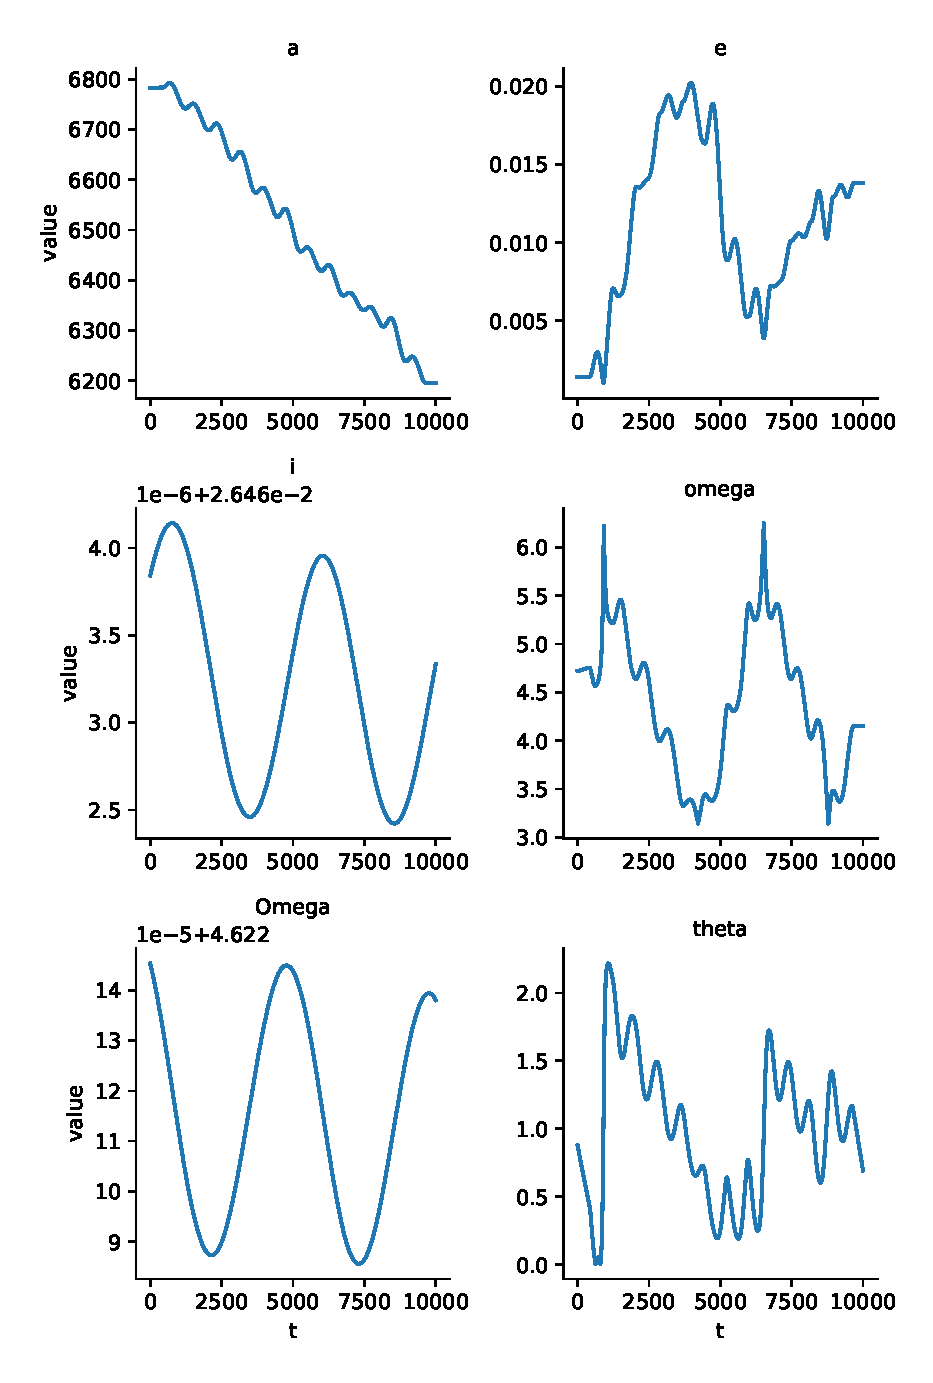
\includegraphics[width=0.85\textwidth]{../Figure/Q2/orbital_elements_variation_moon_10000}
    \caption{Variation of Parameter due to moon gravity perturbation for 10000 seconds}
\end{figure}